\documentclass[../../relatorio.tex]{subfiles}

\begin{document}

\subsection{Taxa Básica de Juros (SELIC)}

\begin{figure}[ht]
  \begin{minipage}{0.70\textheight}
    \centering
      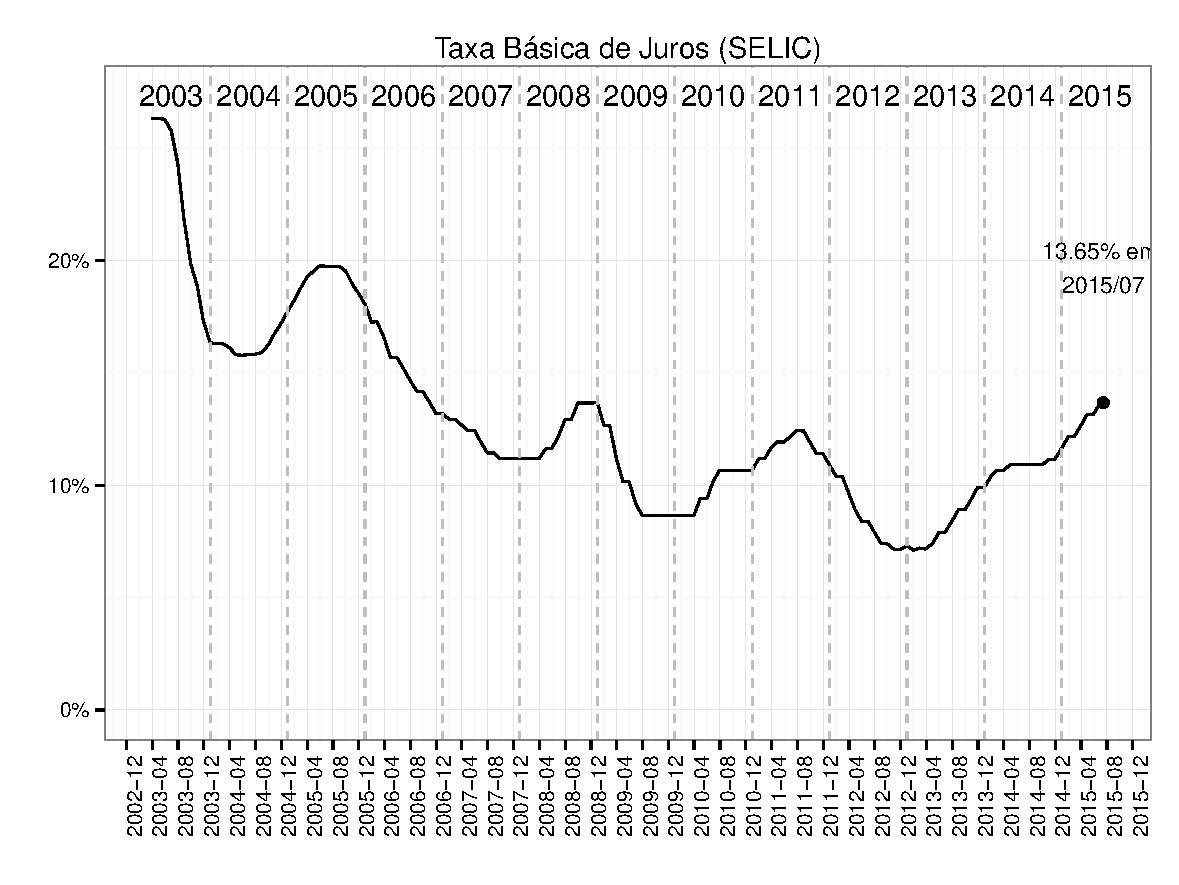
\includegraphics[width=17cm]{Juros.pdf}
  \end{minipage}
\end{figure}

A \textbf{taxa SELIC} é um índice pelo qual as taxas de juros cobradas pelo mercado se balizam no Brasil. É a taxa básica utilizada como referência pela política monetária.

A taxa overnight do Sistema Especial de Liquidação e de Custódia (SELIC), expressa na forma anual, é a taxa média ponderada pelo volume das operações de financiamento por um dia, lastreadas em títulos públicos federais e realizadas no SELIC, na forma de operações compromissadas.

A meta para a taxa SELIC é estabelecida pelo Comitê de Política Monetária (Copom).

Segundo o portal
Infomoney\footnote{http://www.infomoney.com.br/minhas-financas/noticia/125180/entenda-que-como-selic-afeta-economia-brasileira-seu-bolso}, esta taxa é usada para operações de curtíssimo prazo
entre os bancos, que, quando querem tomar recursos emprestados de outros
bancos por um dia, oferecem títulos públicos como lastro, visando
reduzir o risco, e, conseqüentemente, a remuneração da transação.

Assim, como o risco final da transação acaba sendo efetivamente o do
governo, pois seus títulos servem de lastro para a operação e o prazo é
o mais curto possível, ou apenas um dia, esta taxa acaba servindo de
referência para todas as demais taxas de juros da economia.

Esta taxa não é fixa e varia praticamente todos os dias, mas dentro de
um intervalo muito pequeno, já que, na grande maioria das vezes, ela
tende a se aproximar da meta da Selic, que é determinada mensalmente
pelo Copom.

Por ser de curtíssimo prazo e por refletir o risco do governo, a Selic
acaba servindo de referência para todas as demais taxas da economia. Em
situações normais a Selic é a taxa mais baixa, o que, porém, não ocorre
sempre. De forma geral, quanto maior o prazo maior o risco e, portanto,
maior a taxa.

Esse não é o caso, porém, quando o governo está adotando uma política
monetária restritiva, com o objetivo de conter a inflação. Neste caso a
taxa pode ser maior do que as taxas de longo prazo, o que indica que o
mercado acredita que a política econômica adotada irá reduzir a
inflação, levando à queda dos juros de longo prazo.

\pagebreak
\end{document}
